\subsection{Trajectory Smoothing}
Trajectory smoothing method is normally used if the whole dataset is given as a whole. Then the path of the robot can be further optimized using this method. In this section, the focus is on the optimization capability of trajectory smoothing method.

Four different sources of data are used and processed as the prediction and measurement including GPS data, IMU data, Odometry data, and gyro data. In the following discussion, three modifications of the data are discussed including filtering odometry data with gyro data, filting GPS data with IMU data, and filtering odometry data is used as the prediction step and modified GPS data is used for correction measurement.

\subsubsection{Gyrodometry}
Before processing the datasets, ``gyrodometry" method is introduced in \cite{borenstein1996gyrodometry} referenced to determine the fused yaw angle change \(\Delta \psi\). One simple experiment is implemented to test on this method. The  bot  was  moved  along  a  groundtruth trajectory (Fig. \ref{fig:odometry_traj}), and the raw sensing data \(n_R\), \(n_L\), and \(\dot{\psi}_{IMU}\) were logged. \(R_R\), \(R_L\), and \(b\) were provided in the parameter sheet.

Based on the data measured on the robot, the yaw angle and angular velocity from pure wheel odometry and IMU, as well as their difference are shown in Fig. \ref{fig:odometry_angle_diff}. According to the figure, the typical range of the \(\dot{\psi}\) difference is within \(\pm\)0.5 rad/s. And the difference between \(\psi\) is generated mainly during the turning process, where the typical \(\dot{\psi}\) difference is within \(\pm\)0.3 rad/s. These show that a meaningful \(C_{\dot{\psi}}\) will be between 0-0.5 rad/s.

The gyrodometry was run on different \(C_{\dot{\psi}}\). According to the result in Fig. \ref{fig:odometry_tune}, always using yaw information from IMU leads to drift in the straight line period, while always using yaw information from wheel odometry leads to larger errors during turning. Choosing \(C_{\dot{\psi}} = 0.2\) rad/s will combine the strength of both the wheel odometry and IMU, and lead to result closer to the ground truth. Therefore, the \(C_{\dot{\psi}}\) is fixed, and the onboard result with this threshold is shown in Fig. \ref{fig:odometry_traj}.

\begin{figure}[hbt!]
    \centering
    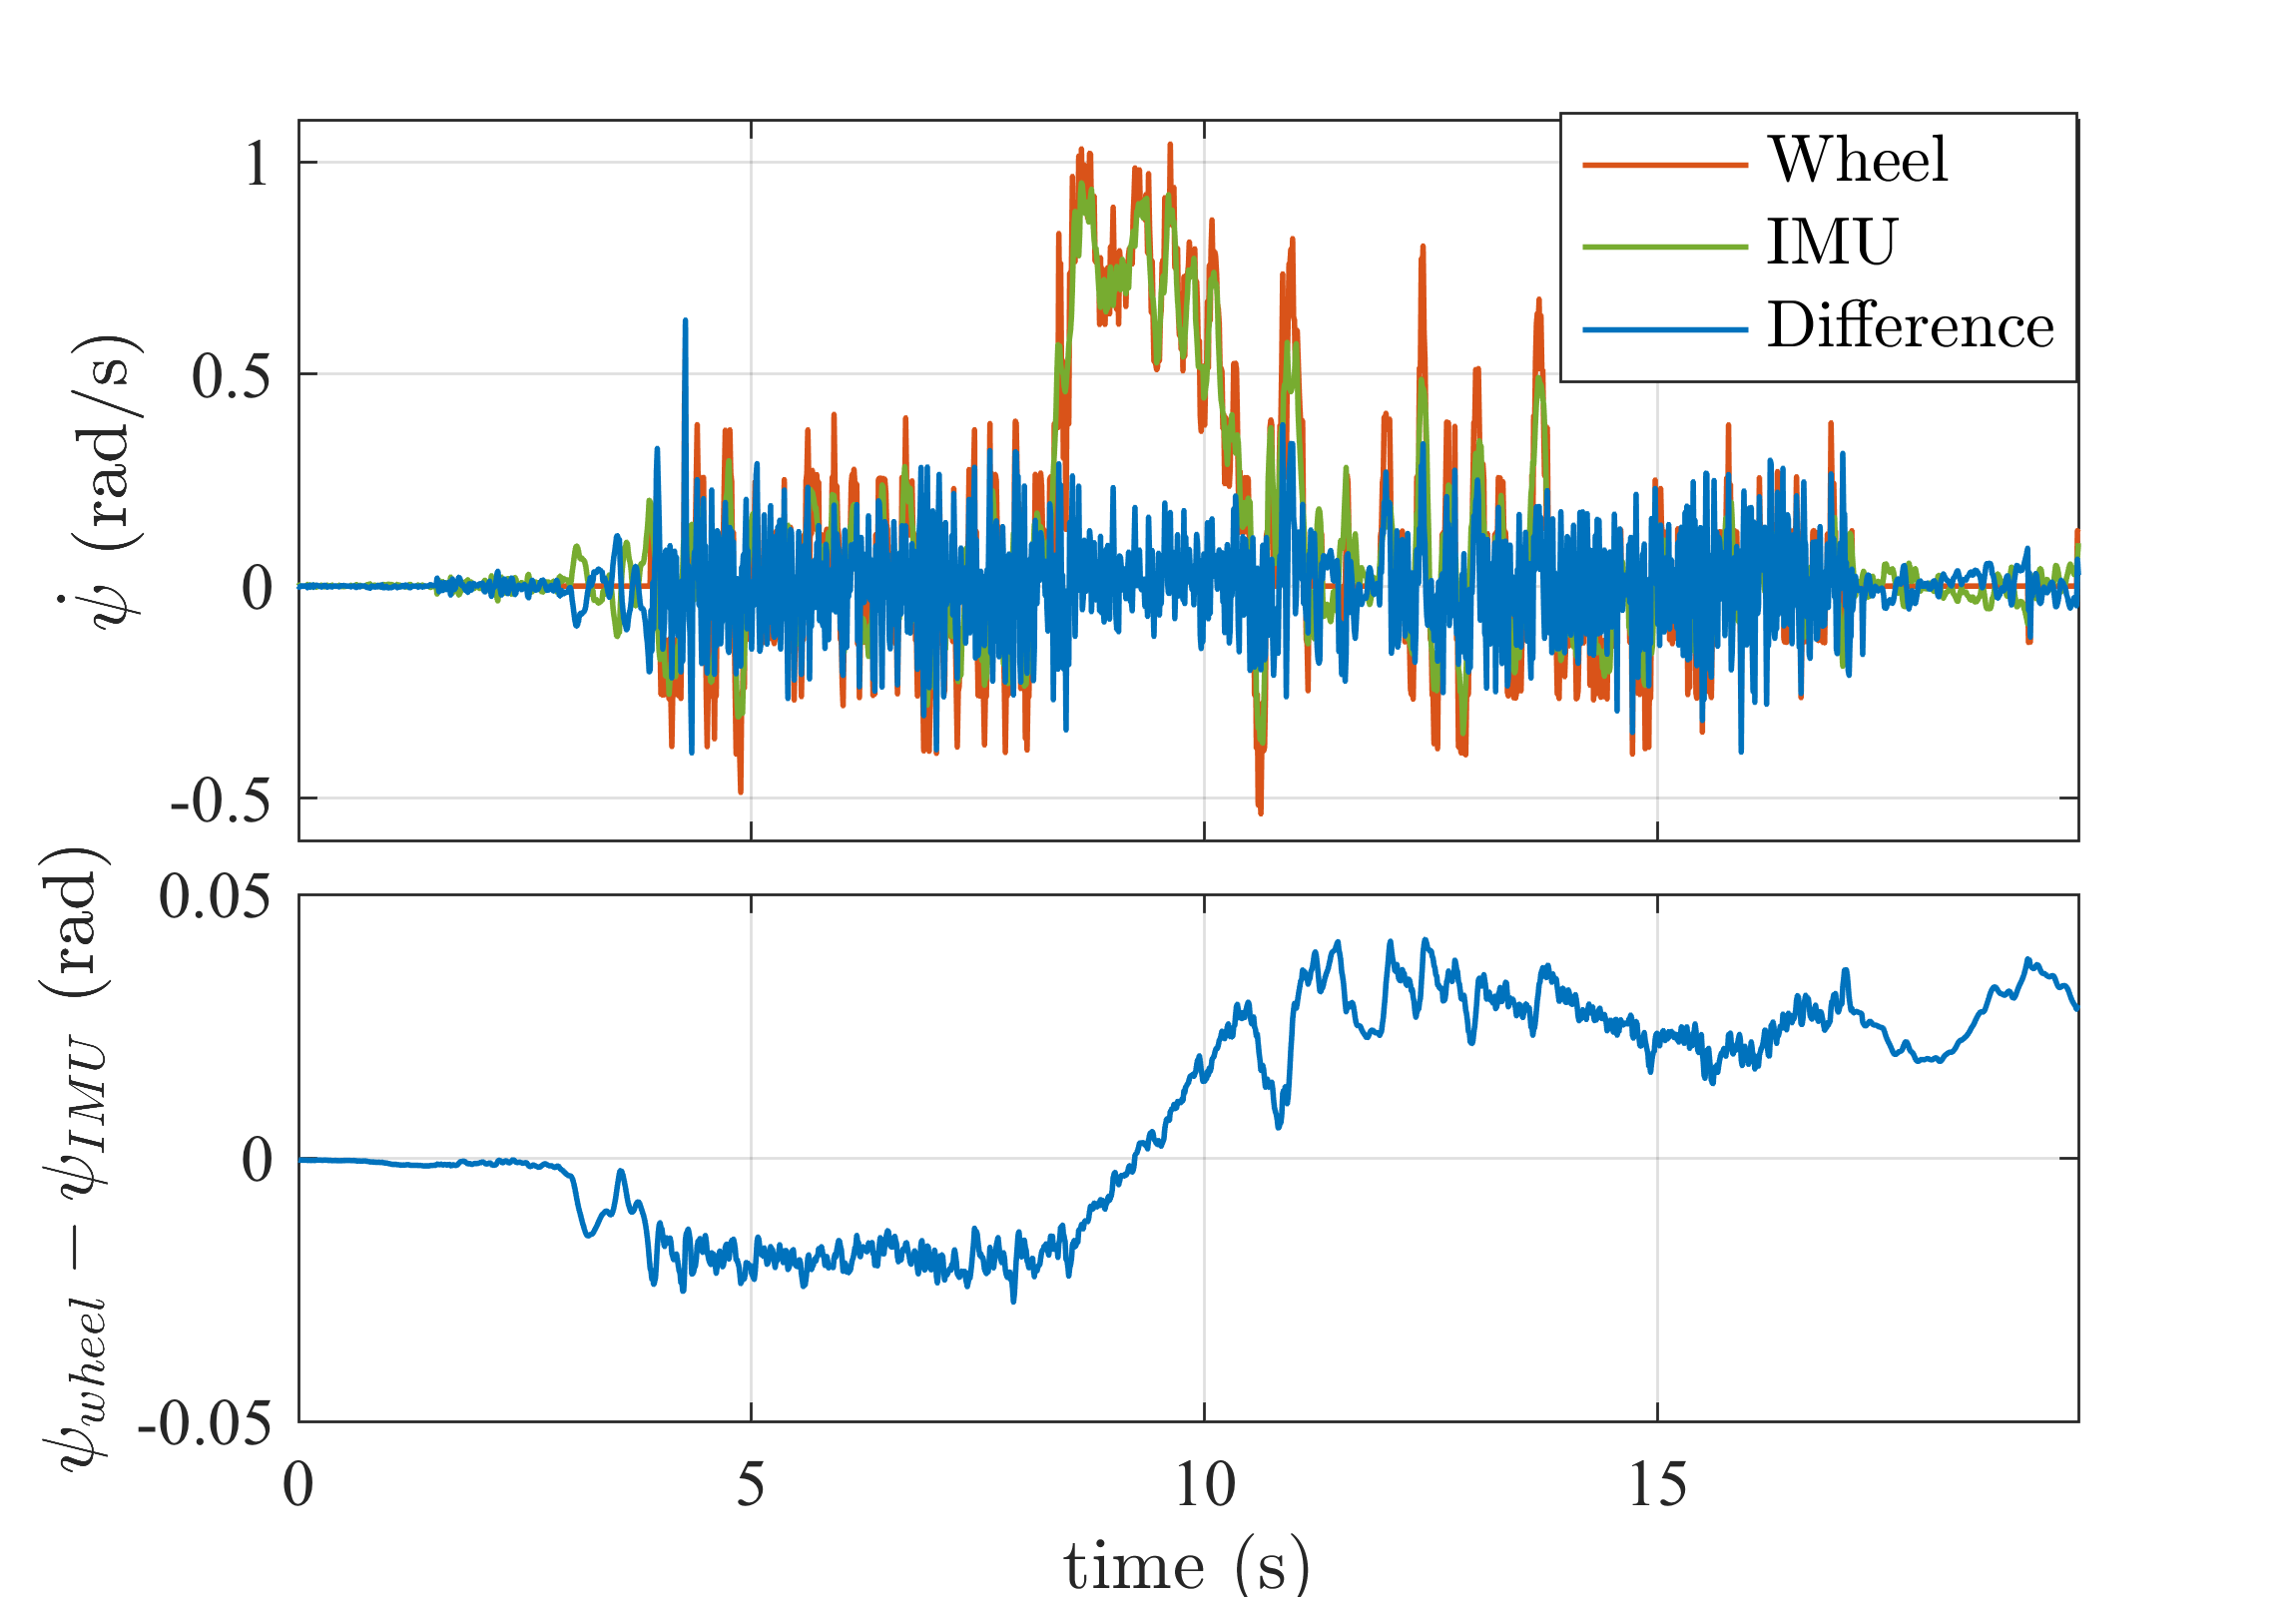
\includegraphics[width = 1.0\linewidth]{media/odometry_angle_diff.png}
    \caption{Yaw angle and angular velocity from wheel odometry and gyro.}
    \label{fig:odometry_angle_diff}
\end{figure}

\begin{figure}[hbt!]
    \centering
    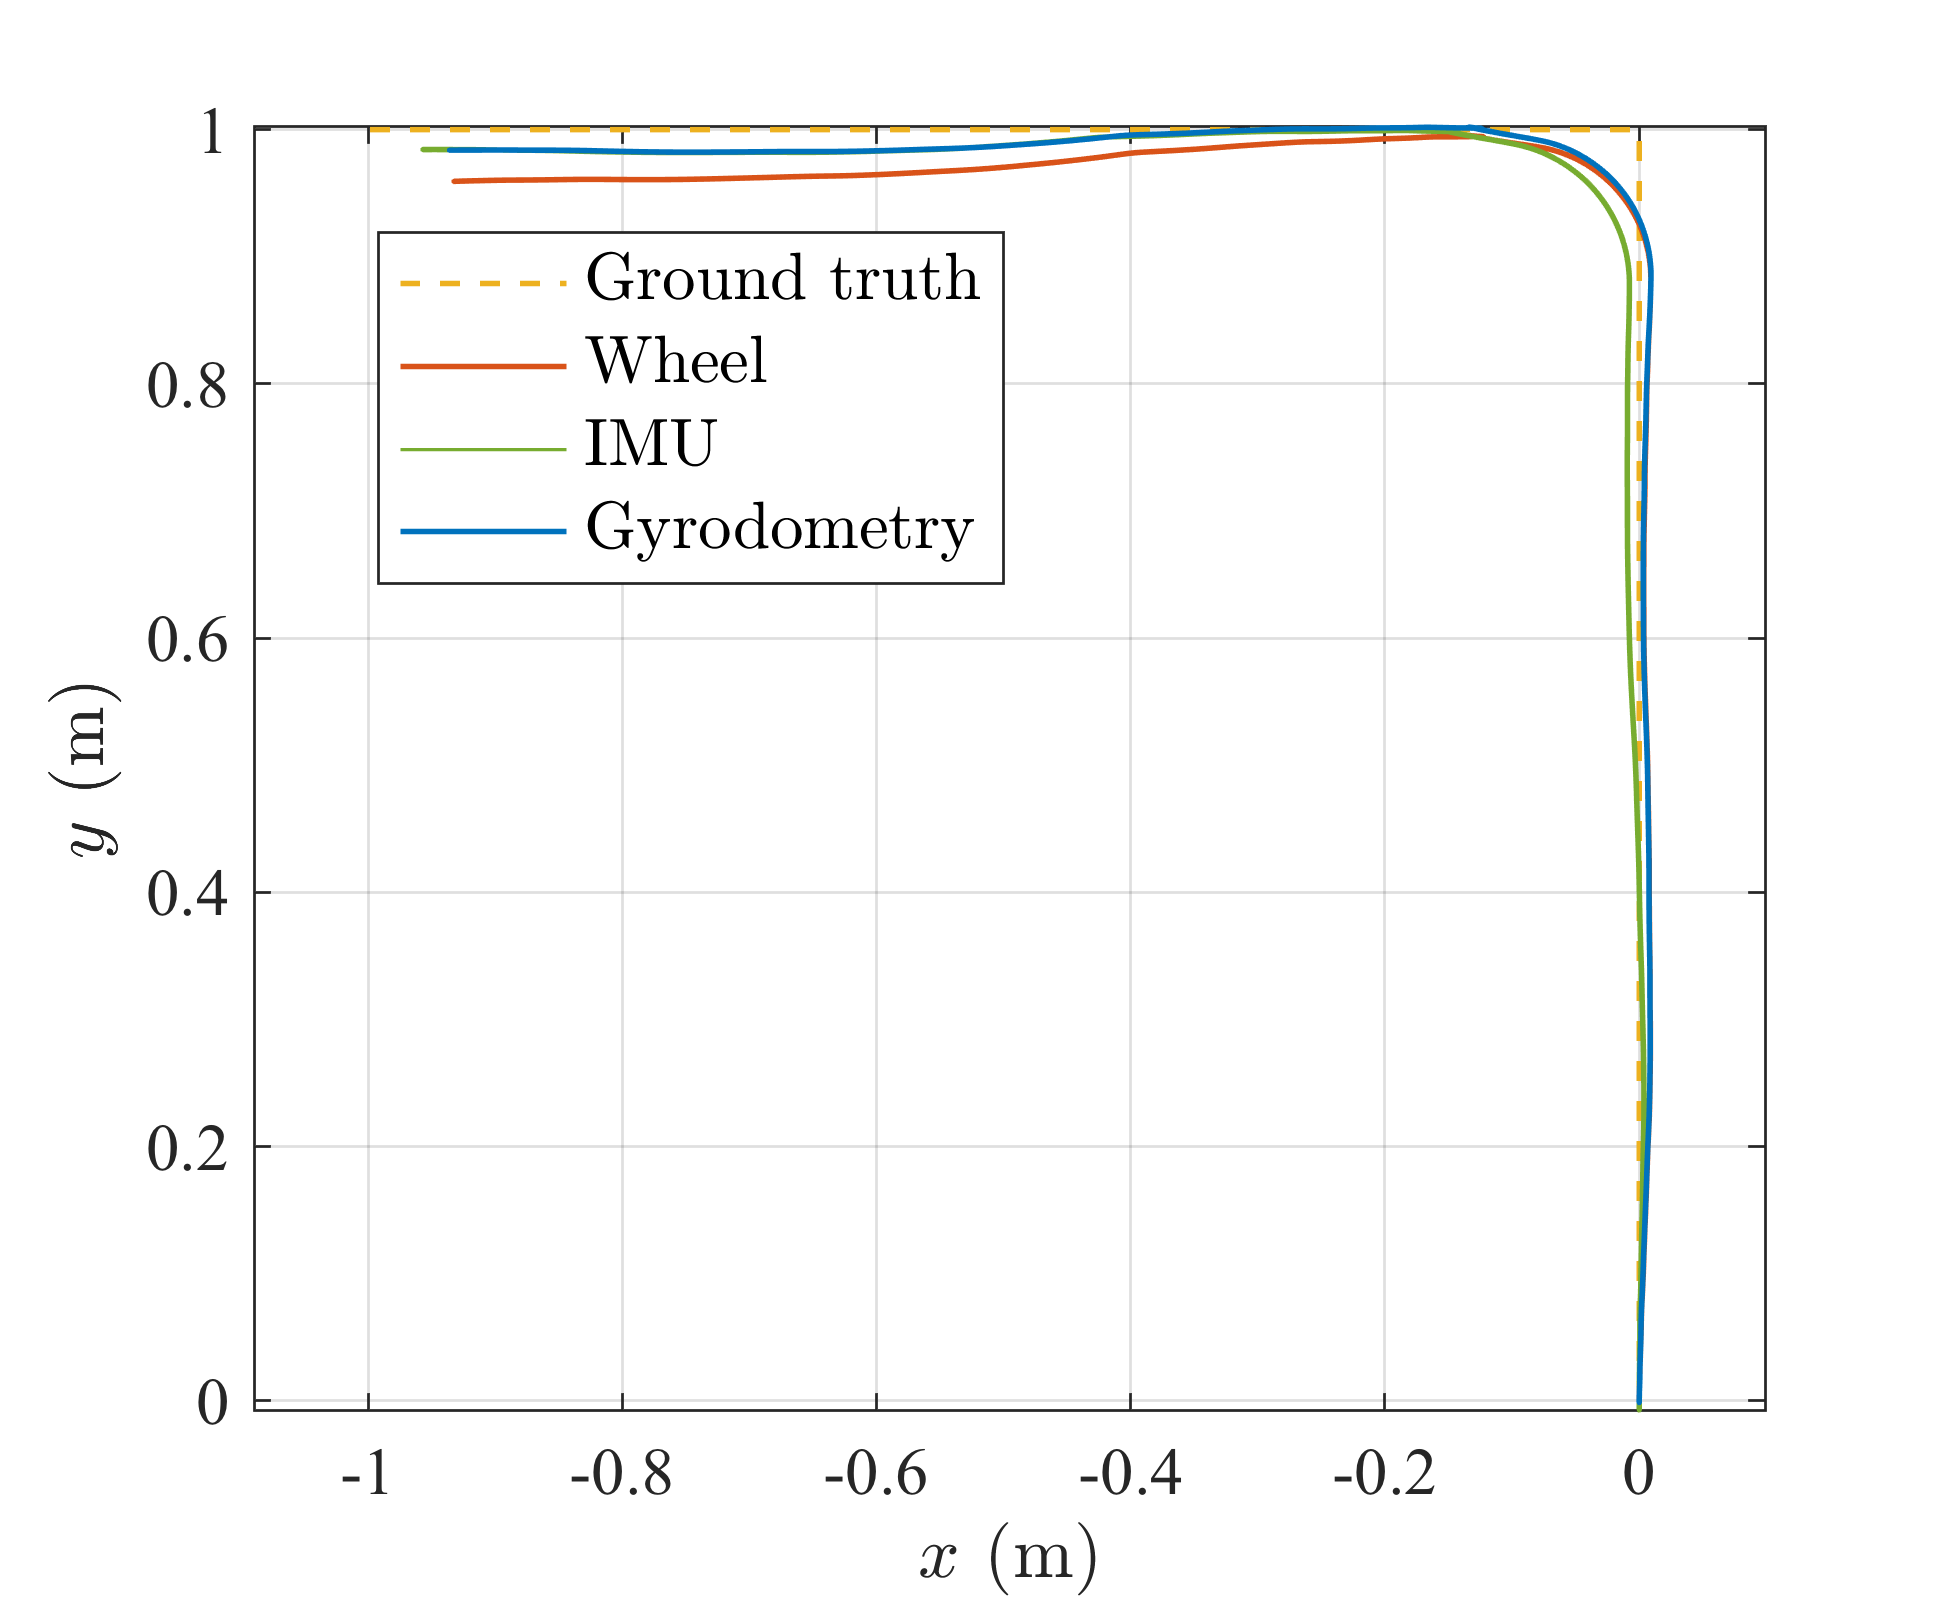
\includegraphics[width = 0.9\linewidth]{media/odometry_traj.png}
    \caption{Odometry results in different modes. The ground truth might be inaccurate during the turning process.}
    \label{fig:odometry_traj}
\end{figure}

\begin{figure}[hbt!]
    \centering
    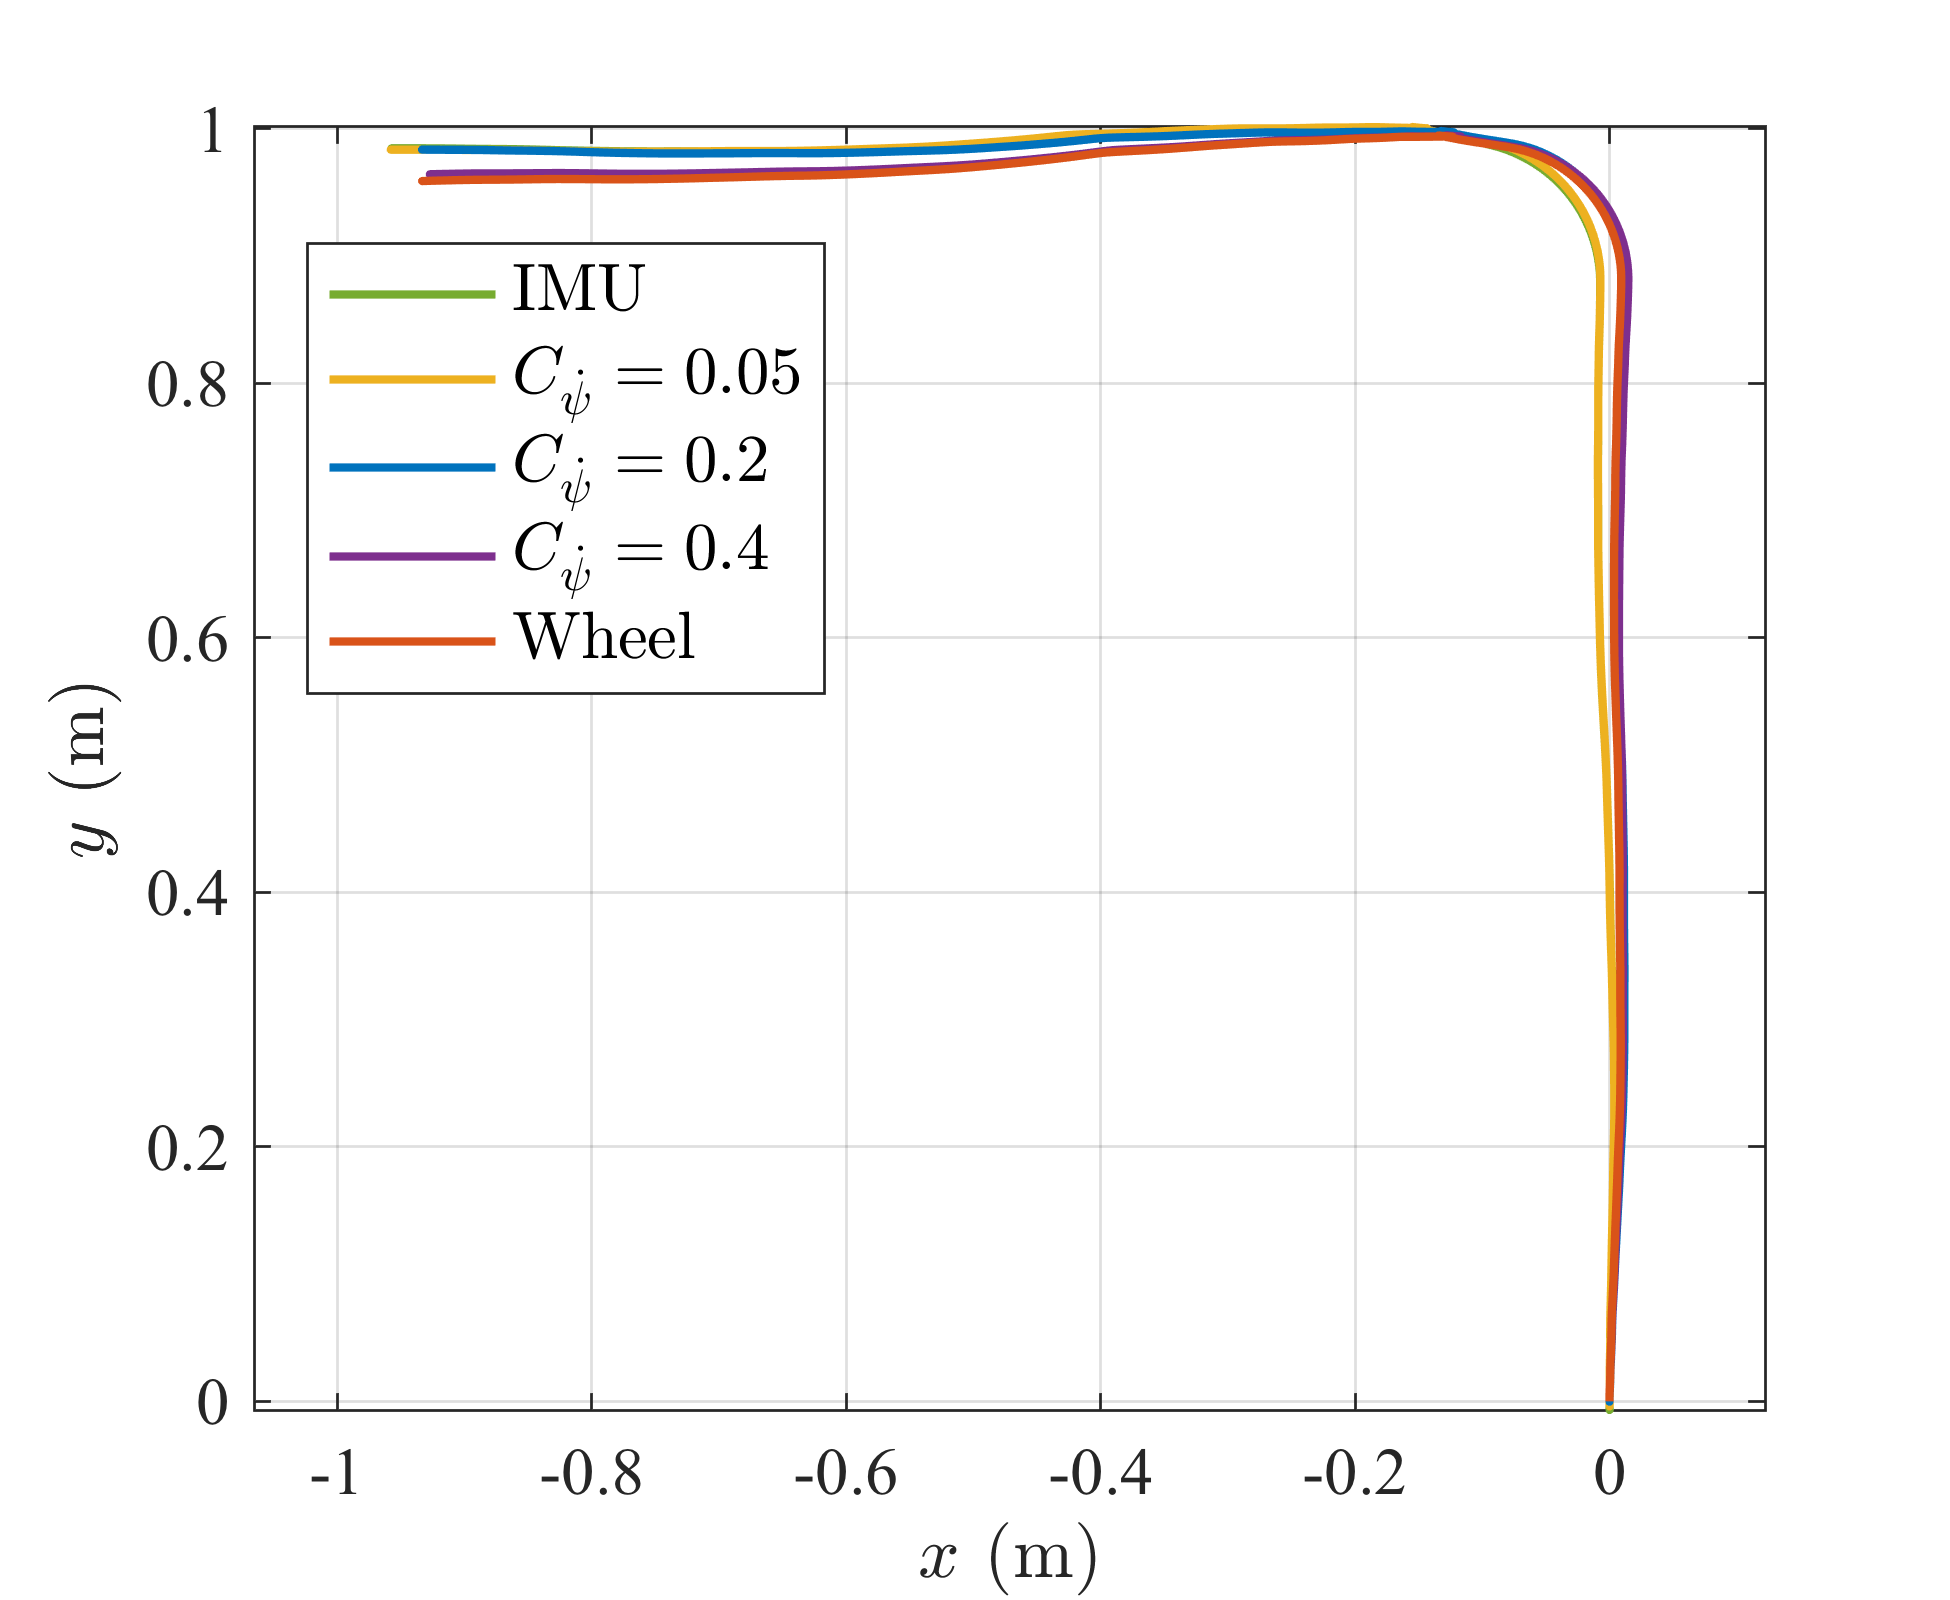
\includegraphics[width = 1.0\linewidth]{media/odometry_tune.png}
    \caption{Gyrodometry results with different \(C_{\dot{\psi}}\) (unit: rad/s) computed in MATLAB. The line of ``IMU" overlaps with ``\(C_{\dot{\psi}}\) = 0.05".}
    \label{fig:odometry_tune}
\end{figure}\label{sec:gyrodo}

\subsubsection{Odometry Fused with Gyroscope}
Now, the next step is to compute a valid set of data using odometry and gyro data. By the nature of the data type, odometry data is accurate for robot moving in a linear motion, but is inaccurate when the robot is turning due to wheel slippage. In contrast, gyro data is a good resource for estimating the turning angle, but performs poorly in linear motion. Thus, two optimization methods are given to combine odometry and gyro data.

One method labelled ``gyro-only" method in Figure \ref{fig:Gyrodometry} is to take odometry data as the prediction of the distance, whereas the FOG information \(\dot{\psi}_{\text{IMU}}\) is used for predicting the heading of the robot. 

One other optimization is the ``gyrodometry" method discribed in section.\ref{sec:gyrodo}. Besides, by experiment, the threshold value is set where \(C_{\dot{\psi}} = 0.2\)

\begin{figure}
    \centering
    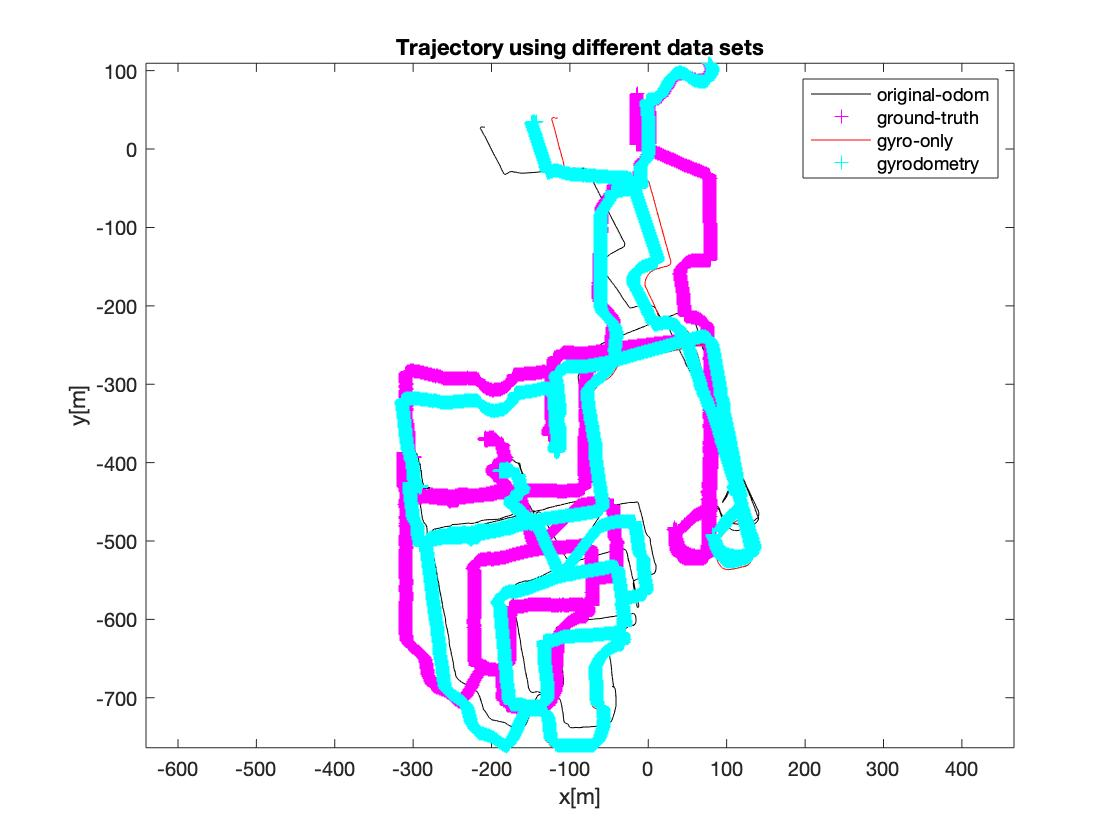
\includegraphics[width=0.8\columnwidth]{media/Gyrodometry.jpg}
    \caption{Odometry optimization using Gyrodometry method}
    \label{fig:Gyrodometry}
\end{figure}

\subsubsection{GPS Optimization using IMU}
GPS data is normally used as the measurement in the outside environment. However, by visualizing the GPS data in Figure \ref{fig:IMU-GPS}, the data contains a lot of outliers(shift in the location). Similar to previous methods where gyro data has been used for the correction of odometry data, IMU data is used to correct the orientation of the GPS data.

Notably, the method used to filter GPS data is incremental Smoothing and Mapping Using the Bayes Tree(ISAM2) describe in \cite{5979641}. After optimization, filtered GPS data is illustrate in Figure \ref{fig:filteredgps}.

\begin{figure}[hbt!]
    \centering
    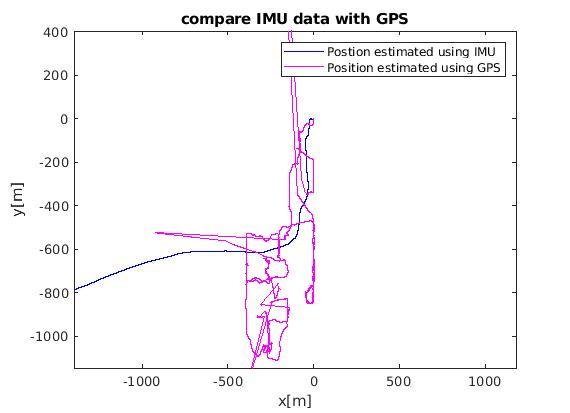
\includegraphics[width = 0.8\linewidth]{media/original-compare.jpg}
    \caption{\textit{Compare IMU data with GPS data.}}
    \label{fig:IMU-GPS}
\end{figure}

\begin{figure}[hbt!]
    \centering
    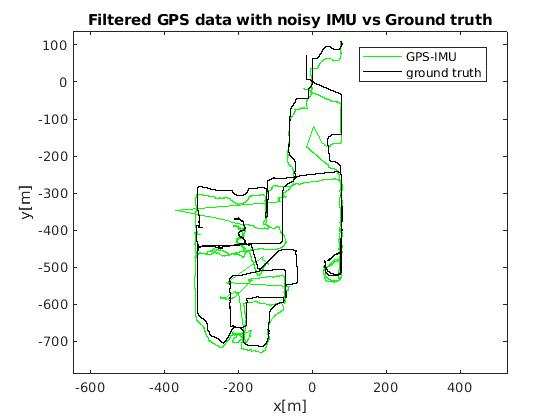
\includegraphics[width = 0.8\linewidth]{media/filteredfGPS.jpg}
    \caption{\textit{GPS data filted by IMU data.}}
    \label{fig:filteredgps}
\end{figure}

\subsubsection{Filtered Odometry with Filtered GPS}
After the filtered odometry data and filtered GPS data are obtained, in this project the last step of the trajectory smoothing is to combine these two data sets together. The method used in this case is ISAM2 in \cite{5979641}.

The steps taken are similar to those in processing GPS data. It is noticeable that the odometry obtained from Figure \ref{fig:Gyrodometry} can be a good metric for orientation, as the details of filtered odometry are similar to those of the ground truth. In contrast, the absolution position of the filtered GPS data is similar to that of the ground truth. By tuning the covariance values($\sigma$) in linear and angular direction, the final filtered graph is shown in Figure \ref{fig:Final plot}.

\begin{figure}[hbt!]
    \centering
    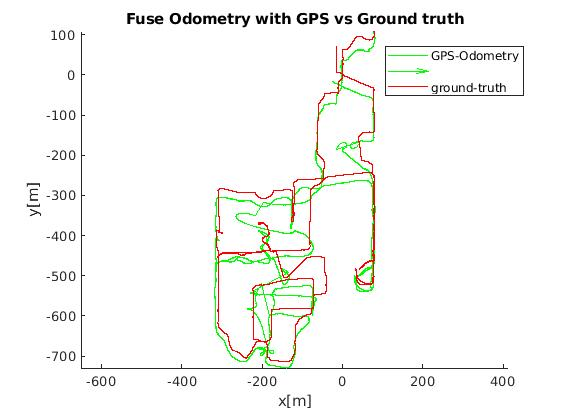
\includegraphics[width = 0.8\linewidth]{media/GPS+Odometry3.jpg}
    \caption{\textit{Compare filtered data with ground truth.}}
    \label{fig:Final plot}
\end{figure}

\subsection{Left Invariant Extended Kalman Filter}


The theory of invariant observer design, based on the estimation error being invariant under the action of a matrix Lie Group, has recently been developed to Invariant EKF, which is applied to simultaneous localization and mapping in \cite{hartley2018contact}. This section derives a Left Invariant EKF to estimate the pose of the robot in the world frame using IMU and GPS measurements. The state is modelled as:

\begin{equation}
    X_{k} = 
    \begin{bmatrix}
    R_{k} & v_{k} & p_{k} \\
    0 & 1 & 0 \\
    0 & 0 & 1
    \end{bmatrix}
\end{equation}

where $R_{k} \in SO(3)$ is the orientation, $v_{k} \in \mathbb{R}^3$ is the linear velocity, and $p_{k} \in \mathbb{R}^3$ is the global position. IMU measurements are used for prediction and GPS measurements are used for correction.

In prediction, the angular acceleration ($w_{k} \in \mathbb{R}^3$) and linear acceleration $a_{k} \mathbb{R}^3$ obtained from the IMU are utilized as input to propagate the state mean using the following equations:

\begin{equation}
    R_{k+1}=R_{k}exp(\overline{\omega_{k}}\delta t)
\end{equation}

\begin{equation}
    v_{k+1}=v_{k}+R_{k}(\overline{\omega_{k}}\delta t)\overline{a_{k}}\delta t+g \delta t
\end{equation}

\begin{equation}
    p_{k+1}=p_{k}+v_{k}+R_{k}(\overline{\omega_{k}}\delta t)\overline{a_{k}}\delta t^{2}+(1/2)g \delta t
\end{equation}

The dynamics above does not consider the in-run bias in the accelerometer, given the fact that only $\pm$0.04 mg bias exists. In order to propagate the covariance, the adjoint operator is obtained as follows:

\begin{equation}
    Ad = 
    \begin{bmatrix}
    R & 0 & 0   \\
    (v)_{\times}R & R & 0  \\
    (p)_{\times}R & 0 & R 
    \end{bmatrix}
\end{equation}

where $()_{\times}$ denotes a $3 \times 3$ skew-symmetric matrix. 
The left-invariant error dynamics depend on the IMU inputs, which are assumed to be constant (following a zero-order hold) between $t_{k}$ and $t_{k+1}$. The state transition matrix for this specified case is determined as:

\begin{equation}
    \phi(t_{k+1},t_{k}) = exp(A \delta t)
\end{equation}

where $A$ is given as:

\begin{equation}
    A = 
    \begin{bmatrix}
    -\bar{\omega_{k}^{\wedge}} & 0 & 0  \\
    -\bar{a_{k}^{\wedge}} & -\bar{\omega_{k}^{\wedge}} & 0 \\
    0 & I & -\bar{\omega_{k}^{\wedge}}
    \end{bmatrix}
\end{equation}

In the correction step, GPS measurements are incorporated in the form:

\begin{equation}
    Y_{k}=\bar{X_{k}}b+V_{k}
\end{equation}

which can be written in the matrix form as:

\begin{equation}
    \begin{bmatrix}
    y_{k} \\
    0 \\
    1
    \end{bmatrix}
    =
    \begin{bmatrix}
    \bar{R_{k}} & \bar{v_{k}} & \bar{p_{k}} \\
    0 & 1 & 0 \\
    0 & 0 & 1
    \end{bmatrix}
    \begin{bmatrix}
    0\\
    0\\
    1
    \end{bmatrix}
    +
    \begin{bmatrix}
    v_{k}\\
    0\\
    0
    \end{bmatrix}
\end{equation}

Using the Left-Invariant EKF equations, H is obtained as:

\begin{equation}
H = 
    \begin{bmatrix}
    0 & 0 & I_{3}
    \end{bmatrix}
\end{equation}

The belief mean ($\bar{X_{t_{k}}^+}$) and covariance ($\bar{P_{t_{k}}^+}$) are then updated with the following equations: 

\begin{equation}
\bar{X}_{t_{k}}^+ = \bar{X}_{t_{k}}^+ 
exp(L_{tk} (\bar{X}_{t_{k}}^{-1}Y_{t_k}-b) )
\end{equation}

\begin{equation}
\bar{P}_{t_{k}}^+ = (I - L_{t_k} H )P_{t_k}(I - L_{t_k} H )^T
+L_{t_k}\bar{N}_{k}L_{t_k}^T
\end{equation}

where 
\begin{equation}
L_{t_k} = P_{t_{k}} H^T S^{-1}
\end{equation}

\begin{equation}
S = HP_{t_k} H^T + \bar{N}_{k}
\end{equation}

The IMU measurements are sampled at 100 Hz, while the GPS measurements are sampled at 10 Hz. We resampled the IMU measurements to 10Hz to match the frequency of GPS measurements and reduce filter runtime.

Although the InEKF algorithm deals with 3D data and states, our implementation focuses only on the x-y position of the robot. Figure \ref{fig:imugps-20s} and Figure \ref{fig:imugps-40s} show the first 20 and 40 seconds of the path, respectively. Figure \ref{fig:imugps-40s} shows the results from the Left-InEKF filter without the prediction step, which means only GPS measurements are used. Both plots show that the results from the filter match accordingly with the GPS data with a maximum difference less than 0.5 meter. The validity of the Left-InEKF filter is proved.

\begin{figure}[hbt!]
    \centering
    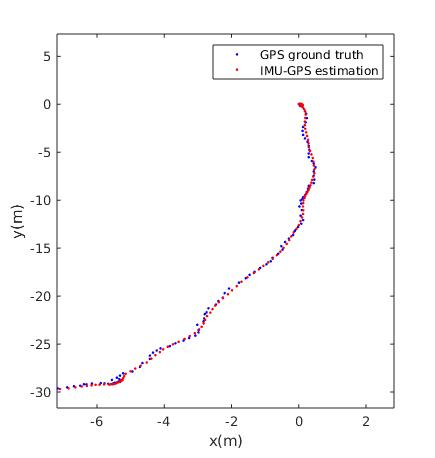
\includegraphics[width = 0.5\linewidth]{media/Starting_results.jpg}
    \caption{Comparison between the IMU-GPS estimation and GPS ground truth in the first 20 secs of data collection}
    \label{fig:imugps-20s}
\end{figure}

\begin{figure}[hbt!]
    \centering
    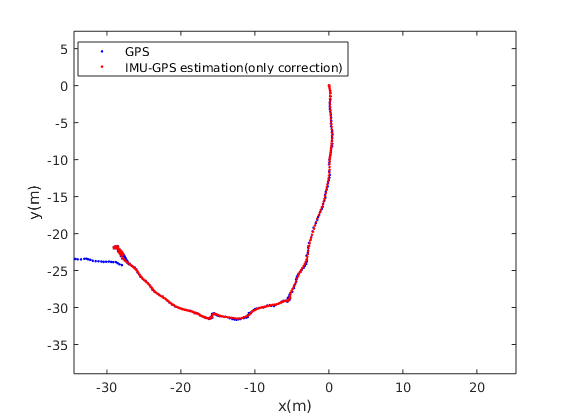
\includegraphics[width = 0.8\linewidth]{media/OnlyGPS.png}
    \caption{Comparison between the filter estimation using only the GPS correction and GPS ground truth in the first 40 secs of data collection}
    \label{fig:imugps-40s}
\end{figure}

Figure \ref{fig:complete_IMUGPS_result} compares the pose estimation from the filter with the ground truth. The starting position of the ground truth is set at the origin.

\begin{figure}[hbt!]
    \centering
    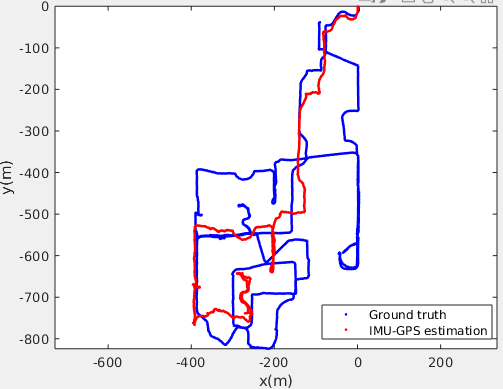
\includegraphics[width = 0.8\linewidth]{media/Complete_InEKF_Result.png}
    \caption{Comparison between the IMU-GPS estimation and the ground truth. About half of the dataset has been processed by the LI-EKF.}
    \label{fig:complete_IMUGPS_result}
\end{figure}

